\epigraph{\textit{'I've got 99 problems, but a pitch ain't one.'}}{Ice-T (1993)}

\section{Optimal control of pitch/travel with LQ control (10.3)}

%%%%%%%%%%%%%%%%%%%%%%%%%%%%%%%%%%%%%%%%%%%%%%%%%%%%%%%%%%%%
\subsection{LQ controller (10.3.1)}
%%%%%%%%%%%%%%%%%%%%%%%%%%%%%%%%%%%%%%%%%%%%%%%%%%%%%%%%%%%%

We introduce feedback to our system using the following manipulated variable:

\begin{equation}
	\V{u}_k = \V{u}_k^* - \M{K} \transpose (\V{x}_k - \V{x}_k^*)
\end{equation}

where $u_k^*$ and $x_k^*$ are the optimal input sequence and optimal trajectory calculated in the previous task. $\M{K}$ is the gain matrix, and can be calculated in numerous ways. We are going to determine it with an LQ (linear quadratic) controller that minimises the function

\begin{equation} \label{eq:LQcost}
	J = \sum\limits_{i=0}^{\infty} \Delta \V{x}_{i+1} \transpose \M{Q} \Delta \V{x}_{i+1} + \Delta \V{u}_{i} \transpose \M{R} \Delta \V{u}_{i}, \quad \M{Q} \geq 0, \, \M{R} > 0
\end{equation}
for the linear model

\begin{equation}
	 \Delta \V{x}_{i+1} = \M{A} \Delta \V{x}_{i} + \M{B} \Delta \V{u}_{i}
\end{equation}
where $\Delta \V{x} = \V{x} - \V{x}^*$ and $\Delta \V{u} = \V{u} - \V{u}^*$ are the deviations from the optimal trajectory. \eqref{eq:LQcost} can be solved in MATLAB using the function \texttt{dlqr}. 

\begin{figure}[H]
	\centering
	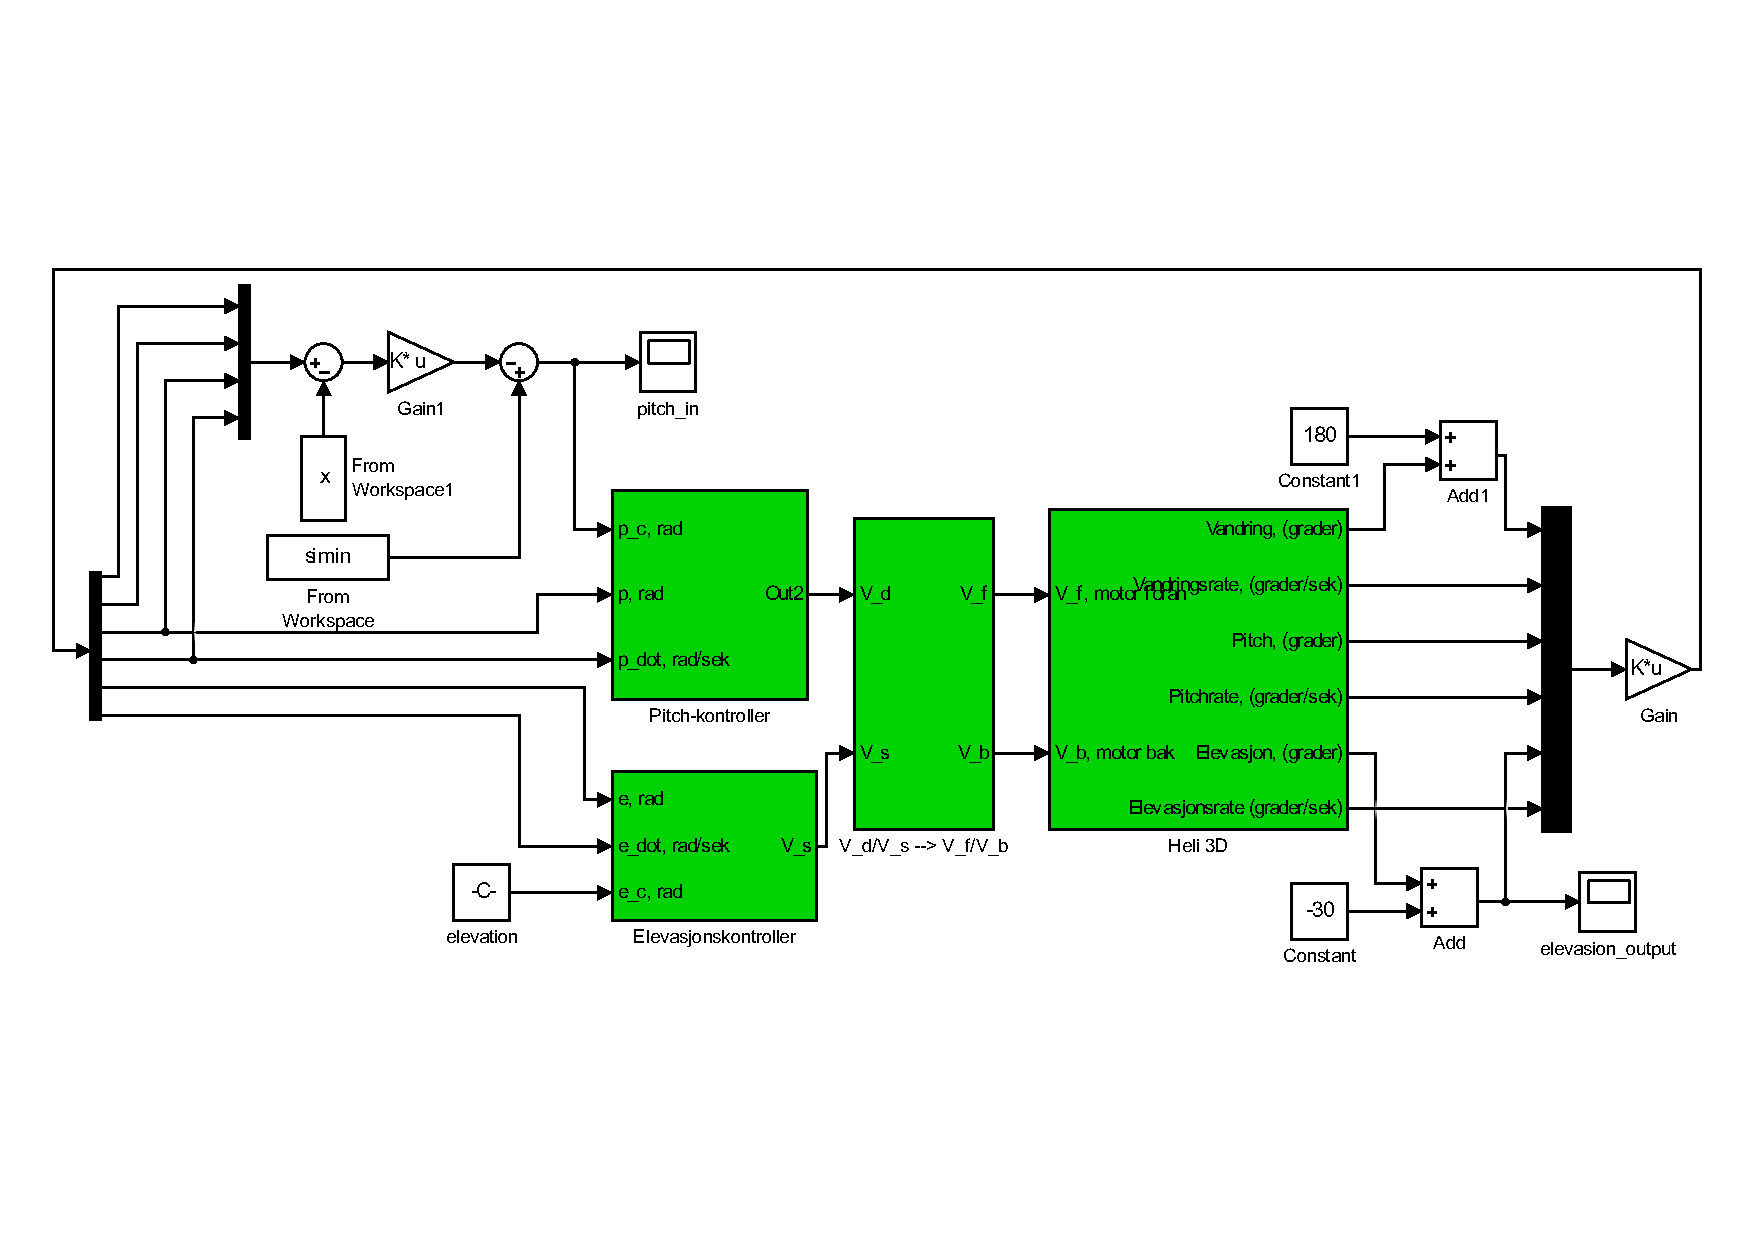
\includegraphics[width=\textwidth, trim=2cm 5cm 2cm 2cm]{simulinkmodels/heldag3}
	\caption{Simulink model of the system}
	\label{fig:heldag3}
\end{figure}

The behaviour of the helicopter is tuned by altering $\M{Q}$ and $R$, and by trial and error we obtained the following values: (TODO: HOW GOOD WAS THIS?)

\begin{equation}
	\M{Q} = 
    \begin{bmatrix}
    	25 & 0 & 0 & 0 \\
        0 & 0.5 & 0 & 0 \\
        0 & 0 & 100 & 0 \\
        0 & 0 & 0 & 0.5
    \end{bmatrix}
\end{equation}

\begin{equation}
	R = 1
\end{equation}

%%%%%%%%%%%%%%%%%%%%%%%%%%%%%%%%%%%%%%%%%%%%%%%%%%%%%%%%%%%%
\subsection{Behaviour with feedback (10.3.2)}
%%%%%%%%%%%%%%%%%%%%%%%%%%%%%%%%%%%%%%%%%%%%%%%%%%%%%%%%%%%%

The first thing we notice is that the helicopter now does come to a halt at the setpoint. In the plots of the measured states, you can see that the travel value is stationary from 19 seconds onwards. You can also see that travel overshoots very slightly, but stabilises nicely at $\lambda_f$.

\begin{figure}[H]
	\centering
	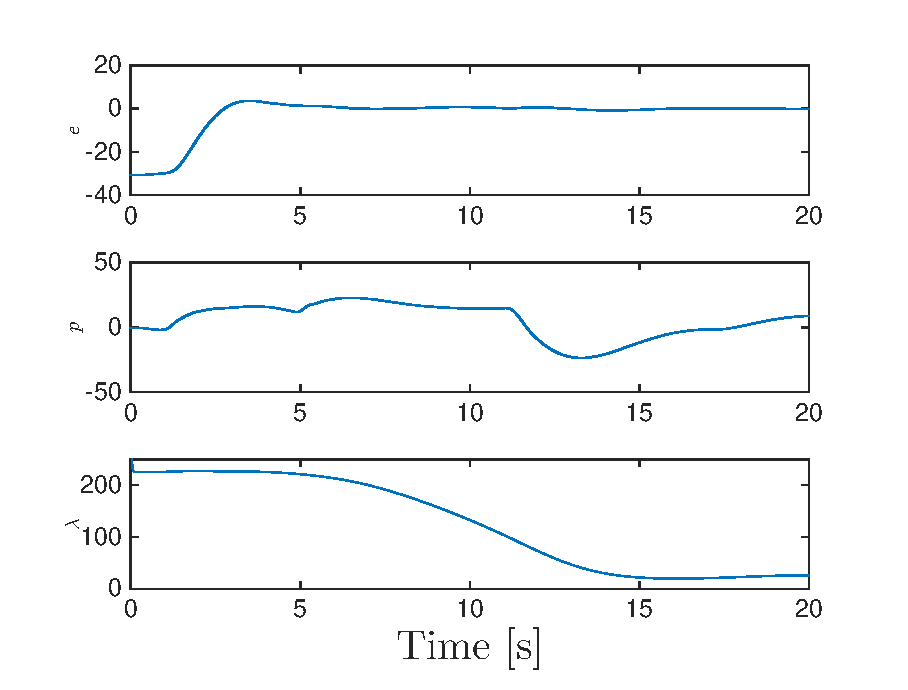
\includegraphics[width=\textwidth]{day3}
	\caption{Actual values day 3}
	\label{fig:day3}
\end{figure}


As shown the shape of both the travel and pitch match the calculated values found in \ref{fig:day2q1} well. The feedback distorts the pitch from the calculated optimal as it works in parallel with the optimal input for the helikopter.

%%%%%%%%%%%%%%%%%%%%%%%%%%%%%%%%%%%%%%%%%%%%%%%%%%%%%%%%%%%%
\subsection{MPC discussion (10.3.3)}
%%%%%%%%%%%%%%%%%%%%%%%%%%%%%%%%%%%%%%%%%%%%%%%%%%%%%%%%%%%%

%%%%%%%%%%%%%%%%%%%%%%%%%%%%%%%%%%%%%%%%%%%%%%%%%%%%%%%%%%%%
\subsubsection{Realization of MPC (10.3.3)}
%%%%%%%%%%%%%%%%%%%%%%%%%%%%%%%%%%%%%%%%%%%%%%%%%%%%%%%%%%%%
MPC can be realized with the following algorithm for linear MPC with state feedback

\begin{algorithmic}
\For{t = 0,1,2,...}
\State Get the current state $x_t$
\State Solve the convex QP problem on the prediction horizon from $t$ to $t+N$ with $x_t$ as the initial condition
\State Apply the first control move $u_t$ from the solution above
\EndFor
\end{algorithmic}

%%%%%%%%%%%%%%%%%%%%%%%%%%%%%%%%%%%%%%%%%%%%%%%%%%%%%%%%%%%%
\subsubsection{Advantages and disadvantages of using MPC (10.3.3)}
%%%%%%%%%%%%%%%%%%%%%%%%%%%%%%%%%%%%%%%%%%%%%%%%%%%%%%%%%%%%
There are both advantages and disadvantages with using an MPC controller compared to LQR.   
MPC requires a lot of computation, and may therefore require more expensive hardware or longer computation time. However, this can yield a very accurate controller. LQR is less computationally intensive, but also less accurate.

%%%%%%%%%%%%%%%%%%%%%%%%%%%%%%%%%%%%%%%%%%%%%%%%%%%%%%%%%%%%
\subsubsection{Figure 8 with MPC (10.3.3)}
%%%%%%%%%%%%%%%%%%%%%%%%%%%%%%%%%%%%%%%%%%%%%%%%%%%%%%%%%%%%
\begin{figure}[H]
	\centering
	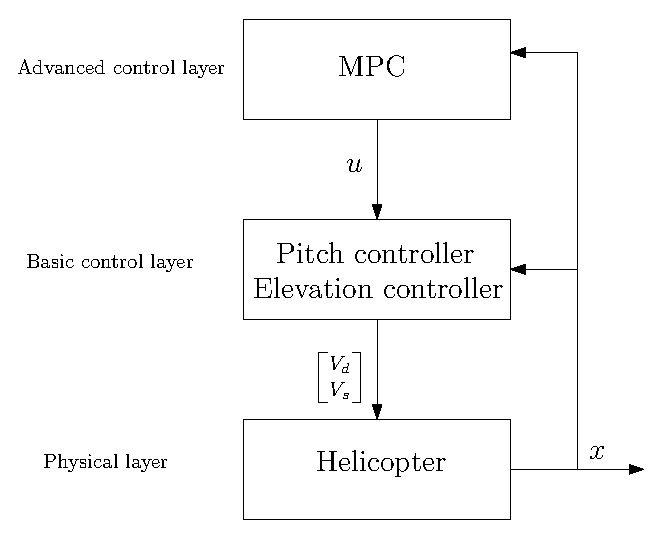
\includegraphics[width=10cm]{figurate_with_MPC}
	\caption{Figure 8 with MPC}
	\label{fig:figurate}
\end{figure}

The MPC, the pitch controller, and the elevation controller receives the measured position $x$ from the helicopter and calculates the input $u$, which the pitch and elevation controllers then use to find the voltages $V_d$ and $V_s$ to control the motors
